% first example chapter
% @author Jan Robert Rösler 
%
\chapter{Navigation mit Bilddaten}

\section{Ansätze}
\note{Hier werden Paper vorgestellt, die Geschichte der Navigation auf Bilddaten und wie das fumktiojneiren kann --> Ansätze}

Versuche durch Verarbeitung von reinen Bilddaten in einem Szenario zu navigieren, gabe es bereits 1989 \cite{pomerleau1989alvinn}.


\begin{figure}
	\centering
	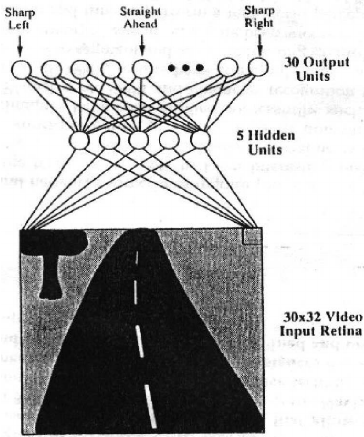
\includegraphics[scale=0.7]{figures/Architecture-ALVINN.png}
	\caption{Das ist eine Abbildung von \cite{Architecture-ALVINN}}
	\label{img:ALVINN}
\end{figure}

 Präsentation ALVINN, dann gegenüberstellung mit modernem Netzwerk a la NVIDIA.

Kurzer Blick auf  Self driving car steering angle4 prediction und berkeley (large scale video sets)




